\newcounter{layer}
\setcounter{layer}{0}
\def\wid{3.7}

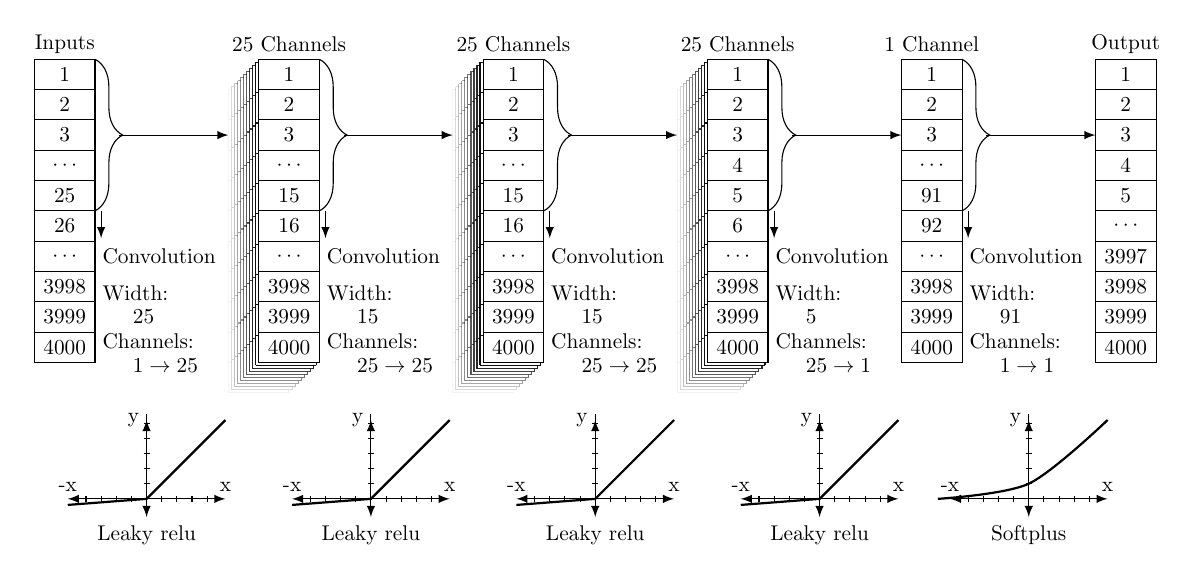
\begin{tikzpicture}[
    scale=.77,
    every node/.style={scale=.77}]

% Layer 1
\begin{scope}[xshift=\thelayer*\wid cm]
\node at (0,0) {Inputs};
\foreach \i [count=\xi] in {1,2,3,$\cdots$,25,26,$\cdots$,3998,3999,4000} {
    \node at(0, -\xi/2) [draw, minimum width = 1cm, minimum height = .5cm] {\i};
}

\draw [decorate,decoration={brace,amplitude=10pt}] (.5,-.25) -- (.5,-2.75);
\draw [-latex] (.6, -2.75) -- (.6, -3.2);
\draw [-latex] (.9, -1.5) -- (\wid - 1, -1.5);
\begin{scope}[xshift=.5cm, yshift=-3.5cm]
\node at (0, 0) [right] {Convolution};
\node at (0,  -.6) [right] {Width:};
\node at (.5, -1) [right] {25};
\node at (0, -1.4) [right] {Channels:};
\node at (.5, -1.8) [right] {$1\rightarrow25$};
\end{scope}
\end{scope}
\stepcounter{layer}

% Layer 2
\begin{scope}[xshift=\thelayer*\wid cm]
\node at (0,0) {25 Channels};
% Backing
\foreach \i in {.5,.45,.4,.35,.3,.25,.2,.15,.1,.05} {
	\begin{scope}[xshift=-.5cm-\i cm, yshift=-.25cm -\i cm]
	\path[fill=white] (0,0) rectangle (1,-5);
	\draw [opacity=1-\i*2 + .05, ystep=.5] (0,0) grid (1,-5);
	\end{scope}
}
\foreach \i [count=\xi] in {1,2,3,$\cdots$,15,16,$\cdots$,3998,3999,4000} {
	\node at(0, -\xi/2) [draw, fill=white, minimum width = 1cm, minimum height = .5cm] {\i};
}

\draw [decorate,decoration={brace,amplitude=10pt}] (.5,-.25) -- (.5,-2.75);
\draw [-latex] (.6, -2.75) -- (.6, -3.2);
\draw [-latex] (.9, -1.5) -- (\wid - 1, -1.5);
\begin{scope}[xshift=.5cm, yshift=-3.5cm]
\node at (0, 0) [right] {Convolution};
\node at (0,  -.6) [right] {Width:};
\node at (.5, -1) [right] {15};
\node at (0, -1.4) [right] {Channels:};
\node at (.5, -1.8) [right] {$25\rightarrow25$};
\end{scope}
\end{scope}
\stepcounter{layer}

% Layer 3
\begin{scope}[xshift=\thelayer*\wid cm]
\node at (0,0) {25 Channels};
% Backing
\foreach \i in {.5,.45,.4,.35,.3,.25,.2,.15,.1,.05} {
	\begin{scope}[xshift=-.5cm-\i cm, yshift=-.25cm -\i cm]
	\path[fill=white] (0,0) rectangle (1,-5);
	\draw [opacity=1-\i*2 + .05, ystep=.5] (0,0) grid (1,-5);
	\end{scope}
}
\foreach \i [count=\xi] in {1,2,3,$\cdots$,15,16,$\cdots$,3998,3999,4000} {
	\node at(0, -\xi/2) [draw, fill=white, minimum width = 1cm, minimum height = .5cm] {\i};
}

\draw [decorate,decoration={brace,amplitude=10pt}] (.5,-.25) -- (.5,-2.75);
\draw [-latex] (.6, -2.75) -- (.6, -3.2);
\draw [-latex] (.9, -1.5) -- (\wid - 1, -1.5);
\begin{scope}[xshift=.5cm, yshift=-3.5cm]
\node at (0, 0) [right] {Convolution};
\node at (0,  -.6) [right] {Width:};
\node at (.5, -1) [right] {15};
\node at (0, -1.4) [right] {Channels:};
\node at (.5, -1.8) [right] {$25\rightarrow25$};
\end{scope}
\end{scope}
\stepcounter{layer}

% Layer 4
\begin{scope}[xshift=\thelayer*\wid cm]
\node at (0,0) {25 Channels};
% Backing
\foreach \i in {.5,.45,.4,.35,.3,.25,.2,.15,.1,.05} {
	\begin{scope}[xshift=-.5cm-\i cm, yshift=-.25cm -\i cm]
	\path[fill=white] (0,0) rectangle (1,-5);
	\draw [opacity=1-\i*2 + .05, ystep=.5] (0,0) grid (1,-5);
	\end{scope}
}
\foreach \i [count=\xi] in {1,2,3,4,5,6,$\cdots$,3998,3999,4000} {
	\node at(0, -\xi/2) [draw, fill=white, minimum width = 1cm, minimum height = .5cm] {\i};
}

\draw [decorate,decoration={brace,amplitude=10pt}] (.5,-.25) -- (.5,-2.75);
\draw [-latex] (.6, -2.75) -- (.6, -3.2);
\draw [-latex] (.9, -1.5) -- (\wid - 1, -1.5);
\begin{scope}[xshift=.5cm, yshift=-3.5cm]
\node at (0, 0) [right] {Convolution};
\node at (0,  -.6) [right] {Width:};
\node at (.5, -1) [right] {5};
\node at (0, -1.4) [right] {Channels:};
\node at (.5, -1.8) [right] {$25\rightarrow1$};
\end{scope}
\end{scope}
\stepcounter{layer}

% Layer 5
\begin{scope}[xshift=\thelayer*\wid cm - .5 cm]
\node at (0,0) {1 Channel};
% Backing
%\foreach \i in {.4,.3,.2,.1} {
%\begin{scope}[xshift=-.5cm-\i cm, yshift=-.25cm -\i cm]
%\path[fill=white] (0,0) rectangle (1,-5);
%\draw [opacity=1-\i*2, ystep=.5] (0,0) grid (1,-5);
%\end{scope}
%}
\foreach \i [count=\xi] in {1,2,3,$\cdots$,91,92,$\cdots$,3998,3999,4000} {
	\node at(0, -\xi/2) [draw, fill=white, minimum width = 1cm, minimum height = .5cm] {\i};
}

\draw [decorate,decoration={brace,amplitude=10pt}] (.5,-.25) -- (.5,-2.75);
\draw [-latex] (.6, -2.75) -- (.6, -3.2);
\draw [-latex] (.9, -1.5) -- (\wid - 1, -1.5);
\begin{scope}[xshift=.5cm, yshift=-3.5cm]
\node at (0, 0) [right] {Convolution};
\node at (0,  -.6) [right] {Width:};
\node at (.5, -1) [right] {91};
\node at (0, -1.4) [right] {Channels:};
\node at (.5, -1.8) [right] {$1\rightarrow1$};
\end{scope}
\end{scope}
\stepcounter{layer}

% Layer Output
\begin{scope}[xshift=\thelayer*\wid cm - 1 cm]
\node at (0,0) {Output};
\foreach \i [count=\xi] in {1,2,3,4,5,$\cdots$,3997,3998,3999,4000} {
	\node at(0, -\xi/2) [draw, fill=white, minimum width = 1cm, minimum height = .5cm] {\i};
}
\end{scope}
\stepcounter{layer}

\begin{scope}[xshift=-.5cm, yshift=-7.5cm]

% Loop as needed
\foreach \i in {\wid * 0.5,\wid * 1.5, \wid * 2.5, \wid * 3.5} {
	\begin{scope}[xshift=\i cm]
	\draw [step=.25] (-1.2, .05) grid (1.2, -.05);
	\draw [step=.25] (-.05, -.2) grid (.05, 1.4);
	\draw [black, latex-latex] (-1.3, 0) node[above] {-x} -- (1.3, 0) node[above] {x};
	\draw [black, latex-latex] (0, -.3)  -- (0, 1.3) node[left] {y};
	\draw [thick, black](-1.3, -.1) -- (0, 0) -- (1.3,1.3);
	\node at (0, -.6) {Leaky relu};
	\end{scope}
}

\begin{scope}[xshift=\wid * 4.5 cm - .25 cm]
\draw [step=.25] (-1.2, .05) grid (1.2, -.05);
\draw [step=.25] (-.05, -.2) grid (.05, 1.4);
\draw [black, latex-latex] (-1.3, 0) node[above] {-x} -- (1.3, 0) node[above] {x};
\draw [black, latex-latex] (0, -.3)  -- (0, 1.3) node[left] {y};
\draw [thick, black, smooth]  plot coordinates {
	(-1.5, 0)
	(0, .25)
	(1.3, 1.3)};
\node at (0, -.6) {Softplus};
\end{scope}

\end{scope}

\end{tikzpicture}